\documentclass[10pt, twocolumn]{article}
\usepackage[margin=0.75in]{geometry}
\usepackage{graphicx}
\usepackage{tikz}
\usepackage{pgfplots}
\usepackage{booktabs}
\usepackage{amsmath}
\usepackage{algorithm}
\usepackage{algorithmic}
\usepackage{hyperref}
\usepackage{xcolor}
\usepackage{caption}
\usepackage{subcaption}
\usepackage{fancyhdr}
\usepackage{enumitem}
\usepackage{listings}
\usepackage{microtype}
\usepackage{orcidlink}
\usepackage{tabularx}
\usepackage{multirow}
\pgfplotsset{compat=1.18}
\usetikzlibrary{arrows.meta, positioning, shapes.geometric, fit, calc, backgrounds, decorations.markings}

% ORCID icon (inline TikZ)
\definecolor{orcidgreen}{HTML}{A6CE39}
\newcommand{\orcidicon}{%
  
\begin{tikzpicture}[baseline=(char.base)]
    \node[circle, fill=orcidgreen, inner sep=0pt, minimum size=2.2ex] (char)
      {\textcolor{white}{\sffamily\bfseries\scriptsize iD}};
  \end{tikzpicture}%
}

% Color palette (same as Paper I for visual continuity)
\definecolor{amblue}{HTML}{2563EB}
\definecolor{amdarkblue}{HTML}{1E40AF}
\definecolor{amteal}{HTML}{0D9488}
\definecolor{amorange}{HTML}{EA580C}
\definecolor{amgray}{HTML}{6B7280}
\definecolor{amlightgray}{HTML}{F3F4F6}
\definecolor{amgreen}{HTML}{059669}
\definecolor{amred}{HTML}{DC2626}
\definecolor{ampurple}{HTML}{7C3AED}

% Listings style
\lstset{
  basicstyle=\ttfamily\scriptsize,
  keywordstyle=\color{amblue}\bfseries,
  commentstyle=\color{amgray}\itshape,
  stringstyle=\color{amteal},
  breaklines=true,
  frame=single,
  rulecolor=\color{amgray!30},
  backgroundcolor=\color{amlightgray},
  numbers=left,
  numberstyle=\tiny\color{amgray},
  tabsize=2
}

% Header
\pagestyle{fancy}
\fancyhf{}
\renewcommand{\headrulewidth}{0.4pt}
\fancyhead[L]{\small\textit{AgenticMemory: Query Expansion}}
\fancyhead[R]{\small\thepage}

\title{\textbf{AgenticMemory~II: Nine Cognitive Query Types for\\Graph-Structured Agent Memory}}
\author{Omoshola Owolabi\,\orcidlink{0009-0006-4089-0732}\\Researcher -- AI/ML\\Agentra Labs\\\texttt{omoshola.owolabi@agentralabs.tech}}
\date{February 22, 2026}

\begin{document}
\maketitle
\thispagestyle{fancy}

% ============================================================================
% ABSTRACT
% ============================================================================
\begin{abstract}
In a companion paper~\cite{owolabi2025agenticmemory}, we introduced AgenticMemory, a binary graph format for persistent AI agent memory with typed cognitive events and semantic edges. That work supported five query types focused on local navigation. We now present AgenticMemory~v0.2.0, extending the query model from 5 to 16~types in four categories: \emph{retrieval} (BM25 text search, hybrid BM25+vector fusion), \emph{structural analysis} (PageRank, degree and betweenness centrality, bidirectional BFS, Dijkstra shortest path), \emph{cognitive reasoning} (counterfactual belief revision, gap detection, analogical pattern matching), and \emph{graph maintenance} (consolidation, drift detection). All nine new algorithms are implemented in 3{,}586~lines of Rust with zero new dependencies. Two new index structures accelerate text queries while maintaining backward compatibility via automatic slow-path fallback and feature flags. The implementation passes 179~Rust and 104~Python tests. Criterion benchmarks on 100{,}000-node graphs show BM25 search at 1.58\,ms (77$\times$ faster than the backward-compatible slow path), hybrid search at 10.83\,ms, PageRank at 34.3\,ms, and bidirectional BFS at 104\,$\mu$s. Computationally intensive queries---gap detection (297\,s), analogical reasoning (229\,s)---scale super-linearly and target periodic batch execution. These additions transform AgenticMemory from a navigable memory store into a cognitive reasoning engine.
\end{abstract}

% ============================================================================
% 1. INTRODUCTION
% ============================================================================
\section{Introduction}
\label{sec:intro}

AgenticMemory~v0.1.0~\cite{owolabi2025agenticmemory} established that AI agent memory is fundamentally a graph navigation problem rather than a text search problem. The binary format---six event types, seven edge types, fixed-size records with memory-mapped $O(1)$ access---demonstrated that a single-file, zero-dependency graph could outperform vector databases, key-value stores, and markdown-based systems across storage efficiency, query latency, and relationship depth.

However, the initial query model was deliberately constrained. The five v0.1 query types---traversal, pattern, temporal, similarity, and resolve---provide local neighborhood exploration and point lookups. They answer questions like ``what caused this decision?'' or ``what is the current version of this fact?'' but cannot answer global structural questions: ``which beliefs are most central to my reasoning?'', ``what decisions lack sufficient evidence?'', or ``has my understanding of this topic drifted over time?''

This paper presents AgenticMemory~v0.2.0, which extends the query model with nine new query types that enable four categories of cognitive capability:

\begin{enumerate}[nosep, leftmargin=*]
  \item \textbf{Retrieval} --- BM25 text search and hybrid BM25+vector fusion via Reciprocal Rank Fusion (RRF) provide keyword-based recall alongside existing embedding-based similarity search.
  \item \textbf{Structural analysis} --- PageRank, degree centrality, betweenness centrality, and shortest-path algorithms (bidirectional BFS for unweighted, Dijkstra for weighted graphs) reveal the topological structure of the agent's knowledge.
  \item \textbf{Cognitive reasoning} --- Counterfactual belief revision, reasoning gap detection, and analogical pattern matching enable the agent to audit its own reasoning processes.
  \item \textbf{Graph maintenance} --- Consolidation (deduplication, contradiction linking, inference promotion) and drift detection enable autonomous knowledge hygiene.
\end{enumerate}

A key engineering constraint is \emph{zero new dependencies}: all algorithms are implemented using only Rust's standard library collections (\texttt{HashMap}, \texttt{BinaryHeap}, \texttt{VecDeque}). This maintains the original design goal of a self-contained binary with no external service requirements.

Backward compatibility is achieved through two mechanisms: (1)~new index structures use tagged blocks that v0.1 readers skip gracefully, and (2)~a feature-flags bitfield in a previously reserved header field allows readers to detect and adapt to format extensions without breaking the fixed-size header layout.

The remainder of this paper is organized as follows. Section~\ref{sec:related} positions this work relative to graph query models and cognitive architectures. Section~\ref{sec:format} describes the format extensions for backward compatibility. Section~\ref{sec:queries} presents the nine new query types with algorithmic details. Section~\ref{sec:evaluation} reports benchmarks on graphs up to 100{,}000 nodes. Section~\ref{sec:sdk} describes the Python SDK extensions. Section~\ref{sec:discussion} discusses implications and limitations. Section~\ref{sec:conclusion} concludes.


% ============================================================================
% 2. RELATED WORK
% ============================================================================
\section{Related Work}
\label{sec:related}

The v0.1 paper~\cite{owolabi2025agenticmemory} surveyed agent memory systems broadly. Here we focus on the specific capabilities that v0.2 adds: text search, graph analysis, and cognitive reasoning over knowledge graphs.

\textbf{BM25 and hybrid search.} BM25~\cite{robertson2009bm25} remains the dominant term-weighting function for information retrieval, outperforming TF-IDF on most benchmarks. Recent work on hybrid search~\cite{lin2021hybrid} combines sparse (BM25) and dense (vector) retrieval using score fusion techniques. Reciprocal Rank Fusion (RRF)~\cite{cormack2009rrf} is a simple, parameter-free method that merges ranked lists by summing $1/(k + r_i)$ across rankings. We adopt RRF for its simplicity and competitive performance.

\textbf{Graph centrality.} PageRank~\cite{page1999pagerank} measures global node importance through iterative random walk simulation. Betweenness centrality~\cite{brandes2001betweenness} quantifies how often a node appears on shortest paths between other nodes. Both have been applied to knowledge graphs for identifying key entities~\cite{angles2008survey}, but not previously to cognitive event graphs where nodes represent agent beliefs rather than real-world entities.

\textbf{Belief revision.} The AGM framework~\cite{alchourron1985agm} formalizes belief revision as contraction and expansion operations on belief sets. Our counterfactual analysis implements a read-only variant: rather than modifying the belief set, we trace the cascade of downstream effects that would result from retracting a given node, enabling ``what if?'' reasoning without mutation.

\textbf{Analogical reasoning.} Structure-mapping theory~\cite{gentner1983structure} proposes that analogies are based on shared relational structure rather than surface similarity. Our analogical query operationalizes this by computing structural fingerprints---in-degree, out-degree, edge type distribution---and combining structural similarity with content similarity to find past reasoning patterns that match a given query pattern.

\textbf{Knowledge graph maintenance.} Entity resolution and deduplication in knowledge graphs is well-studied~\cite{nickel2016review}, but typically requires external embedding models or string similarity services. Our consolidation algorithm operates entirely within the graph, using edge-weighted similarity and content overlap to identify duplicate and contradictory nodes.


% ============================================================================
% 3. FORMAT EXTENSIONS
% ============================================================================
\section{Format Extensions}
\label{sec:format}

The v0.2 format maintains full backward compatibility with v0.1 while adding two new index structures and a feature-flags mechanism.

% ----------------------------------------------------------------------------
\subsection{New Index Structures}

The v0.1 index block used four tagged entries (type index, temporal index, session index, cluster map). The v0.2 format adds two new tags:

\textbf{TermIndex (tag 0x05).} An inverted index mapping terms to posting lists. Each posting list entry stores the node ID, term frequency, and field (content or metadata). The index is built during file write by tokenizing node content with a simple whitespace-and-punctuation tokenizer. This enables the BM25 fast path: queries against the inverted index complete in $O(q \cdot |\text{postings}|)$ time rather than the $O(n)$ full-scan slow path.

\textbf{DocLengths (tag 0x06).} A dense array of \texttt{u32} token counts, one per node, indexed by node ID. This is required for BM25 length normalization: $\text{norm} = 1 - b + b \cdot (dl / \text{avgdl})$, where $dl$ is the document length and $\text{avgdl}$ is the average across all documents. Storing lengths in a contiguous array avoids recomputing them at query time.

% ----------------------------------------------------------------------------
\subsection{Feature Flags}

The v0.1 header reserved 7~bytes at the end of the 64-byte header record. The v0.2 format repurposes 4~of these bytes as a \texttt{u32} feature-flags bitfield:

\begin{itemize}[nosep, leftmargin=*]
  \item Bit~0: \texttt{HAS\_TERM\_INDEX} --- TermIndex block is present.
  \item Bit~1: \texttt{HAS\_DOC\_LENGTHS} --- DocLengths block is present.
  \item Bits~2--31: Reserved for future extensions.
\end{itemize}

The remaining 3~reserved bytes are untouched. This design enables forward compatibility: a v0.1 reader encountering a v0.2 file will read the reserved bytes as zero (which they were in v0.1) and skip unknown index tags during index block parsing. A v0.2 reader opening a v0.1 file detects the absence of feature flags and falls back to slow-path algorithms.

% ----------------------------------------------------------------------------
\subsection{Backward Compatibility}

Compatibility is bidirectional:

\textbf{v0.1 files read by v0.2 code.} When the TermIndex is absent, BM25 and hybrid queries fall back to a slow path that tokenizes node content on-the-fly and computes BM25 scores in a single $O(n)$ pass. This is correct but slower than the indexed fast path. All other new queries (centrality, shortest path, cognitive reasoning, maintenance) operate on the node and edge tables, which are unchanged from v0.1.

\textbf{v0.2 files read by v0.1 code.} The v0.1 reader's index parser skips unknown tag bytes using the length field in each tag-length-value block. The node table, edge table, content block, and feature vectors are identical in layout. The only observable difference is that the reserved header bytes are no longer zero, which v0.1 readers ignore.

% Figure: BM25 dual-path architecture
\begin{figure}[t]
\centering
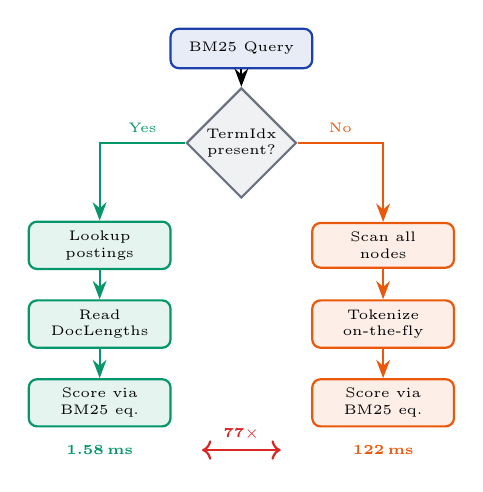
\begin{tikzpicture}[
  every node/.style={font=\tiny},
  box/.style={rectangle, rounded corners=3pt, draw=#1, fill=#1!10, minimum width=1.8cm, minimum height=0.5cm, align=center, thick},
  decision/.style={diamond, draw=amgray, fill=amgray!10, minimum width=1.2cm, minimum height=0.7cm, align=center, thick, font=\tiny, inner sep=1pt},
  arr/.style={-{Stealth}, thick},
]

% Query input
\node[box=amdarkblue] (q) at (0, 0) {BM25 Query};

% Decision
\node[decision] (dec) at (0, -1.2) {TermIdx\\present?};

% Fast path
\node[box=amgreen] (fast1) at (-1.8, -2.5) {Lookup\\postings};
\node[box=amgreen] (fast2) at (-1.8, -3.5) {Read\\DocLengths};
\node[box=amgreen] (fast3) at (-1.8, -4.5) {Score via\\BM25 eq.};
\node[font=\tiny\bfseries, text=amgreen] at (-1.8, -5.1) {1.58\,ms};

% Slow path
\node[box=amorange] (slow1) at (1.8, -2.5) {Scan all\\nodes};
\node[box=amorange] (slow2) at (1.8, -3.5) {Tokenize\\on-the-fly};
\node[box=amorange] (slow3) at (1.8, -4.5) {Score via\\BM25 eq.};
\node[font=\tiny\bfseries, text=amorange] at (1.8, -5.1) {122\,ms};

% Arrows
\draw[arr] (q) -- (dec);
\draw[arr, amgreen] (dec) -- node[above, font=\tiny] {Yes} (-1.8, -1.2) -- (fast1);
\draw[arr, amorange] (dec) -- node[above, font=\tiny] {No} (1.8, -1.2) -- (slow1);
\draw[arr, amgreen] (fast1) -- (fast2);
\draw[arr, amgreen] (fast2) -- (fast3);
\draw[arr, amorange] (slow1) -- (slow2);
\draw[arr, amorange] (slow2) -- (slow3);

% Speedup annotation
\draw[amred, thick, <->] (-0.5, -5.1) -- (0.5, -5.1) node[midway, above, font=\tiny\bfseries, text=amred] {77$\times$};

\end{tikzpicture}
\caption{BM25 dual-path architecture. The fast path (green) uses the TermIndex and DocLengths array for sub-linear query time. The slow path (orange) performs a full scan for backward compatibility with v0.1 files. Measured speedup at 100K nodes: 77$\times$.}
\label{fig:bm25_paths}
\end{figure}

% Figure 1: Format extension diagram
\begin{figure}[t]
\centering
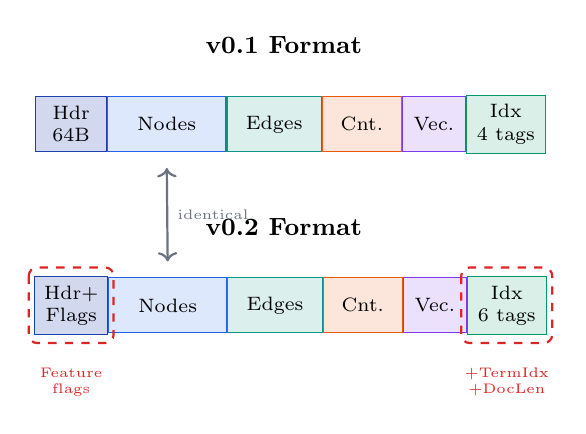
\begin{tikzpicture}[
  every node/.style={font=\scriptsize},
  section/.style={rectangle, draw, minimum height=0.7cm, align=center, font=\scriptsize},
]
% v0.1 format
\node[font=\small\bfseries] at (0, 2.5) {v0.1 Format};
\node[section, fill=amdarkblue!20, draw=amdarkblue, minimum width=0.9cm] (h1) at (-2.7, 1.5) {Hdr\\64B};
\node[section, fill=amblue!15, draw=amblue, minimum width=1.5cm, anchor=west] (n1) at (h1.east) {Nodes};
\node[section, fill=amteal!15, draw=amteal, minimum width=1.2cm, anchor=west] (e1) at (n1.east) {Edges};
\node[section, fill=amorange!15, draw=amorange, minimum width=1.0cm, anchor=west] (c1) at (e1.east) {Cnt.};
\node[section, fill=ampurple!15, draw=ampurple, minimum width=0.8cm, anchor=west] (v1) at (c1.east) {Vec.};
\node[section, fill=amgreen!15, draw=amgreen, minimum width=1.0cm, anchor=west] (i1) at (v1.east) {Idx\\4 tags};

% v0.2 format
\node[font=\small\bfseries] at (0, 0.2) {v0.2 Format};
\node[section, fill=amdarkblue!20, draw=amdarkblue, minimum width=0.9cm] (h2) at (-2.7, -0.8) {Hdr+\\Flags};
\node[section, fill=amblue!15, draw=amblue, minimum width=1.5cm, anchor=west] (n2) at (h2.east) {Nodes};
\node[section, fill=amteal!15, draw=amteal, minimum width=1.2cm, anchor=west] (e2) at (n2.east) {Edges};
\node[section, fill=amorange!15, draw=amorange, minimum width=1.0cm, anchor=west] (c2) at (e2.east) {Cnt.};
\node[section, fill=ampurple!15, draw=ampurple, minimum width=0.8cm, anchor=west] (v2) at (c2.east) {Vec.};
\node[section, fill=amgreen!15, draw=amgreen, minimum width=1.0cm, anchor=west] (i2) at (v2.east) {Idx\\6 tags};

% Highlight new parts
\draw[amred, thick, dashed, rounded corners=3pt] ([xshift=-2pt, yshift=3pt]h2.north west) rectangle ([xshift=2pt, yshift=-3pt]h2.south east);
\draw[amred, thick, dashed, rounded corners=3pt] ([xshift=-2pt, yshift=3pt]i2.north west) rectangle ([xshift=2pt, yshift=-3pt]i2.south east);

\node[font=\tiny, text=amred, align=center] at ([yshift=-0.6cm]h2.south) {Feature\\flags};
\node[font=\tiny, text=amred, align=center] at ([yshift=-0.6cm]i2.south) {+TermIdx\\+DocLen};

% Identical annotation
\draw[amgray, thick, <->] ([yshift=-0.2cm]n1.south) -- ([yshift=0.2cm]n2.north) node[midway, right, font=\tiny, text=amgray] {identical};

\end{tikzpicture}
\caption{Binary format evolution from v0.1 to v0.2. Node table, edge table, content block, and feature vectors are unchanged. The header gains a feature-flags bitfield in previously reserved bytes, and the index block gains two new tagged entries (TermIndex, DocLengths). Red dashes highlight changes.}
\label{fig:format_evolution}
\end{figure}


% ============================================================================
% 4. QUERY EXPANSION
% ============================================================================
\section{Query Expansion: Nine New Query Types}
\label{sec:queries}

The nine new queries are organized into four categories reflecting the cognitive capability they provide. Figure~\ref{fig:query_taxonomy} shows the complete taxonomy of all 16~query types across v0.1 and v0.2.

% Figure 2: Query taxonomy
\begin{figure*}[t]
\centering
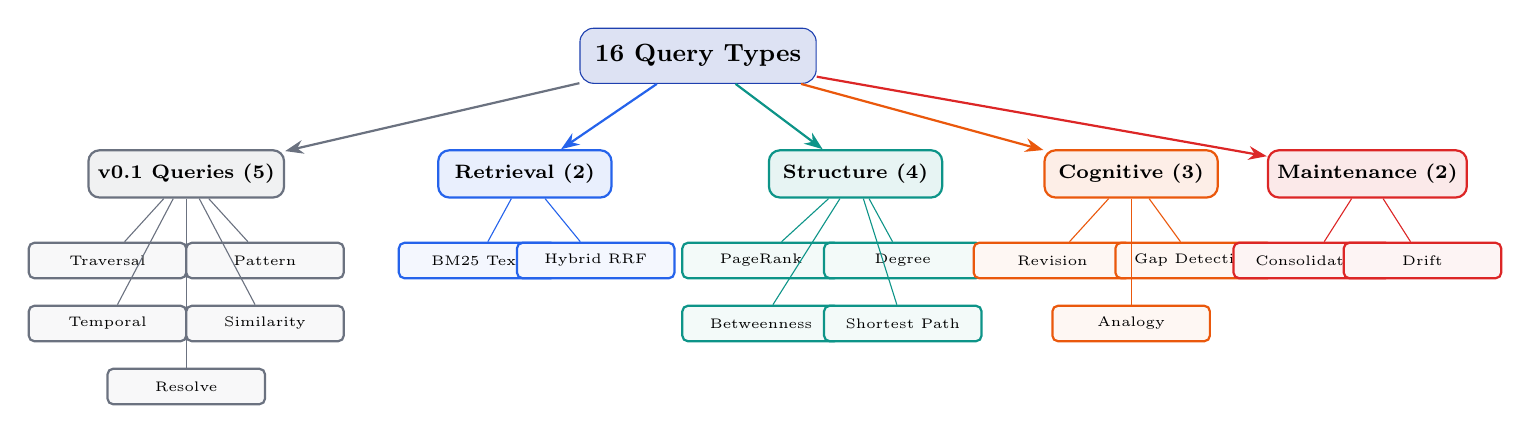
\begin{tikzpicture}[
  every node/.style={font=\scriptsize},
  catbox/.style={rectangle, rounded corners=4pt, draw=#1, fill=#1!10, minimum width=2.2cm, minimum height=0.6cm, align=center, font=\scriptsize\bfseries, thick},
  qbox/.style={rectangle, rounded corners=2pt, draw=#1, fill=#1!5, minimum width=2.0cm, minimum height=0.45cm, align=center, font=\tiny, thick},
  oldbox/.style={rectangle, rounded corners=2pt, draw=amgray, fill=amgray!5, minimum width=2.0cm, minimum height=0.45cm, align=center, font=\tiny, thick},
]

% Root
\node[rectangle, rounded corners=5pt, draw=amdarkblue, fill=amdarkblue!15, minimum width=3cm, minimum height=0.7cm, font=\small\bfseries] (root) at (0, 0) {16 Query Types};

% v0.1 category
\node[catbox=amgray] (v1cat) at (-6.5, -1.5) {v0.1 Queries (5)};
\node[oldbox] (q1) at (-7.5, -2.6) {Traversal};
\node[oldbox] (q2) at (-5.5, -2.6) {Pattern};
\node[oldbox] (q3) at (-7.5, -3.4) {Temporal};
\node[oldbox] (q4) at (-5.5, -3.4) {Similarity};
\node[oldbox] (q5) at (-6.5, -4.2) {Resolve};

% Retrieval
\node[catbox=amblue] (ret) at (-2.2, -1.5) {Retrieval (2)};
\node[qbox=amblue] (q6) at (-2.8, -2.6) {BM25 Text};
\node[qbox=amblue] (q7) at (-1.3, -2.6) {Hybrid RRF};

% Structure
\node[catbox=amteal] (str) at (2.0, -1.5) {Structure (4)};
\node[qbox=amteal] (q8) at (0.8, -2.6) {PageRank};
\node[qbox=amteal] (q9) at (2.6, -2.6) {Degree};
\node[qbox=amteal] (q10) at (0.8, -3.4) {Betweenness};
\node[qbox=amteal] (q11) at (2.6, -3.4) {Shortest Path};

% Cognitive
\node[catbox=amorange] (cog) at (5.5, -1.5) {Cognitive (3)};
\node[qbox=amorange] (q12) at (4.5, -2.6) {Revision};
\node[qbox=amorange] (q13) at (6.3, -2.6) {Gap Detection};
\node[qbox=amorange] (q14) at (5.5, -3.4) {Analogy};

% Maintenance
\node[catbox=amred] (mnt) at (8.5, -1.5) {Maintenance (2)};
\node[qbox=amred] (q15) at (7.8, -2.6) {Consolidation};
\node[qbox=amred] (q16) at (9.2, -2.6) {Drift};

% Connections
\draw[-{Stealth}, amgray, thick] (root) -- (v1cat);
\draw[-{Stealth}, amblue, thick] (root) -- (ret);
\draw[-{Stealth}, amteal, thick] (root) -- (str);
\draw[-{Stealth}, amorange, thick] (root) -- (cog);
\draw[-{Stealth}, amred, thick] (root) -- (mnt);

\foreach \q in {q1,q2} \draw[amgray] (v1cat) -- (\q);
\foreach \q in {q3,q4} \draw[amgray] (v1cat) -- (\q);
\draw[amgray] (v1cat) -- (q5);

\draw[amblue] (ret) -- (q6);
\draw[amblue] (ret) -- (q7);
\foreach \q in {q8,q9,q10,q11} \draw[amteal] (str) -- (\q);
\foreach \q in {q12,q13,q14} \draw[amorange] (cog) -- (\q);
\draw[amred] (mnt) -- (q15);
\draw[amred] (mnt) -- (q16);

\end{tikzpicture}
\caption{Complete query taxonomy for AgenticMemory v0.2. Gray boxes indicate the five v0.1 query types; colored boxes indicate the nine new v0.2 types organized into four cognitive categories.}
\label{fig:query_taxonomy}
\end{figure*}


% ----------------------------------------------------------------------------
\subsection{Retrieval: BM25 Text Search}
\label{sec:bm25}

BM25~\cite{robertson2009bm25} scores each document $d$ against a query $Q = \{q_1, \ldots, q_n\}$ as:

\begin{equation}
\text{BM25}(d, Q) = \sum_{i=1}^{n} \text{IDF}(q_i) \cdot \frac{f(q_i, d) \cdot (k_1 + 1)}{f(q_i, d) + k_1 \cdot (1 - b + b \cdot \frac{|d|}{\text{avgdl}})}
\label{eq:bm25}
\end{equation}

where $f(q_i, d)$ is the term frequency, $|d|$ is the document length in tokens, $\text{avgdl}$ is the average document length, and $\text{IDF}(q_i) = \ln\!\left(\frac{N - n(q_i) + 0.5}{n(q_i) + 0.5} + 1\right)$ with $N$ total documents and $n(q_i)$ documents containing term $q_i$. We use $k_1 = 1.2$ and $b = 0.75$ following standard practice.

\textbf{Fast path.} When the TermIndex is present (Figure~\ref{fig:bm25_paths}), the algorithm iterates over posting lists for each query term, accumulating BM25 scores in a hash map. Document lengths are read from the DocLengths array. Total cost: $O(q \cdot |\text{postings}|)$ where $q$ is the number of query terms.

\textbf{Slow path.} When reading a v0.1 file without indexes (Figure~\ref{fig:bm25_paths}), the algorithm performs a single $O(n)$ pass: tokenize each node's content, compute term frequencies on the fly, and accumulate BM25 scores. This is approximately 77$\times$ slower than the fast path on a 100K-node graph (122\,ms vs.\ 1.58\,ms) but produces identical results.

Both paths support optional filtering by event type and session ID.

% ----------------------------------------------------------------------------
\subsection{Retrieval: Hybrid Search}
\label{sec:hybrid}

Hybrid search combines BM25 (sparse, keyword-based) and cosine similarity (dense, embedding-based) results using Reciprocal Rank Fusion~\cite{cormack2009rrf}:

\begin{equation}
\text{RRF}(d) = \sum_{r \in \mathcal{R}} \frac{1}{k + \text{rank}_r(d)}
\label{eq:rrf}
\end{equation}

where $\mathcal{R}$ is the set of ranking systems (BM25 and vector), $\text{rank}_r(d)$ is the rank of document $d$ in ranking $r$, and $k = 60$ is a constant that dampens the influence of high rankings. RRF is parameter-free (beyond $k$) and does not require score normalization, making it robust across heterogeneous scoring functions.

The hybrid query first executes BM25 and similarity searches independently, then merges the results by RRF score. The output includes both the combined rank and the individual BM25 and vector scores for interpretability.

% ----------------------------------------------------------------------------
\subsection{Structural Analysis: Centrality}
\label{sec:centrality}

Three centrality measures reveal the topological importance of nodes in the agent's knowledge graph:

\textbf{PageRank}~\cite{page1999pagerank} computes stationary probabilities of a random walk with damping factor $\alpha = 0.85$:

\begin{equation}
\text{PR}(v) = \frac{1-\alpha}{N} + \alpha \sum_{u \in B(v)} \frac{\text{PR}(u)}{|L(u)|}
\label{eq:pagerank}
\end{equation}

where $B(v)$ is the set of nodes linking to $v$ and $L(u)$ is the out-degree of $u$. Our implementation handles dangling nodes (nodes with no outgoing edges) by redistributing their rank mass uniformly. Iteration continues until the $L^1$ norm of the rank vector change falls below $10^{-6}$ or 100 iterations are reached.

\textbf{Degree centrality} computes the normalized degree $C_D(v) = \frac{\deg(v)}{N-1}$ for each node, providing a simple measure of local connectivity.

\textbf{Betweenness centrality}~\cite{brandes2001betweenness} measures how often a node appears on shortest paths between other pairs of nodes. We implement Brandes' algorithm, which computes betweenness in $O(VE)$ time by performing a BFS from each source node and accumulating pair-dependencies in a single backward pass. For graphs exceeding 1{,}000 nodes, we use random source sampling (200 sources) to approximate betweenness in practical time.

All centrality queries support optional filtering by event type, allowing the agent to ask questions like ``which facts are most central to my reasoning?'' or ``which decisions are bridge nodes between topic clusters?''

% ----------------------------------------------------------------------------
\subsection{Structural Analysis: Shortest Path}
\label{sec:paths}

Two shortest-path algorithms serve different graph models:

\textbf{Bidirectional BFS} finds the shortest unweighted path between two nodes. The algorithm alternates BFS expansion from the source and target, terminating when the frontiers intersect. This reduces the search space from $O(b^d)$ to $O(b^{d/2})$ where $b$ is the branching factor and $d$ is the path length. A depth limit (default: 20) prevents exhaustive search in disconnected subgraphs.

\textbf{Dijkstra's algorithm} finds the shortest weighted path, using edge weights as distances. The implementation uses a binary heap (\texttt{BinaryHeap<Reverse<(Cost, NodeId)>>}) and returns both the path and its total weight.

Both algorithms return the full node sequence, enabling the agent to understand not just \emph{that} two beliefs are connected but \emph{how} they are connected through intermediate reasoning steps.


% ----------------------------------------------------------------------------
\subsection{Cognitive Reasoning: Belief Revision}
\label{sec:revision}

The belief revision query performs counterfactual analysis: given a target node $v$, it computes the downstream effects of retracting $v$ from the belief graph. This is a \emph{read-only} operation---no nodes or edges are modified.

\begin{algorithm}[t]
\caption{Counterfactual Belief Revision}
\label{alg:revision}
\begin{algorithmic}[1]
\REQUIRE Graph $G = (V, E)$, target node $v$
\ENSURE Cascade set $C$, impact report $R$
\STATE $C \leftarrow \emptyset$; $Q \leftarrow \{v\}$
\WHILE{$Q \neq \emptyset$}
  \STATE $u \leftarrow Q.\text{dequeue}()$
  \FOR{each edge $(u, w, t)$ where $t \in \{\textsc{CausedBy}, \textsc{Supports}\}$}
    \IF{$w \notin C$}
      \STATE $C \leftarrow C \cup \{w\}$
      \STATE Compute impact: $\text{conf\_loss}(w)$, $\text{alt\_support}(w)$
      \IF{$\text{alt\_support}(w) = 0$}
        \STATE $Q.\text{enqueue}(w)$ \COMMENT{No remaining support; propagate}
      \ENDIF
    \ENDIF
  \ENDFOR
\ENDWHILE
\STATE $R \leftarrow$ summarize($C$): affected nodes, confidence losses, unsupported inferences
\RETURN $C, R$
\end{algorithmic}
\end{algorithm}

The algorithm (Algorithm~\ref{alg:revision}, illustrated in Figure~\ref{fig:revision_cascade}) performs a BFS along \textsc{CausedBy} and \textsc{Supports} edges. For each downstream node, it checks whether alternative support exists (other incoming \textsc{Supports} or \textsc{CausedBy} edges from nodes not in the cascade set). Nodes with no remaining support are added to the cascade and their downstream dependencies are explored recursively.

The report includes: (1)~directly affected nodes, (2)~confidence reductions for each affected node, (3)~unsupported inferences that would become unjustified, and (4)~a total impact score. This enables an agent to reason about the consequences of being wrong: ``if this fact is incorrect, what conclusions would I need to reconsider?''

% Figure: Belief revision cascade example
\begin{figure}[t]
\centering
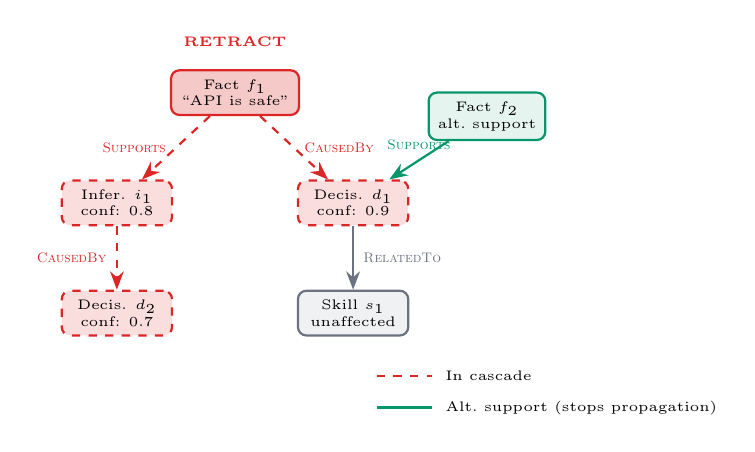
\begin{tikzpicture}[
  every node/.style={font=\tiny},
  node/.style={rectangle, rounded corners=3pt, draw=#1, fill=#1!10, minimum width=1.4cm, minimum height=0.55cm, align=center, thick},
  edge/.style={-{Stealth}, thick},
  cascade/.style={rectangle, rounded corners=3pt, draw=amred, fill=amred!15, minimum width=1.4cm, minimum height=0.55cm, align=center, thick, dashed},
]

% Target node (retracted)
\node[node=amred, fill=amred!25] (f1) at (0, 0) {Fact $f_1$\\``API is safe''};
\node[font=\tiny\bfseries, text=amred] at ([yshift=0.35cm]f1.north) {RETRACT};

% First level downstream
\node[cascade] (i1) at (-1.5, -1.4) {Infer. $i_1$\\conf: 0.8};
\node[cascade] (d1) at (1.5, -1.4) {Decis. $d_1$\\conf: 0.9};

% Alternative support
\node[node=amgreen] (f2) at (3.2, -0.3) {Fact $f_2$\\alt.\ support};

% Second level
\node[cascade] (d2) at (-1.5, -2.8) {Decis. $d_2$\\conf: 0.7};
\node[node=amgray] (s1) at (1.5, -2.8) {Skill $s_1$\\unaffected};

% Edges
\draw[edge, amred, dashed] (f1) -- node[left, font=\tiny] {\textsc{Supports}} (i1);
\draw[edge, amred, dashed] (f1) -- node[right, font=\tiny] {\textsc{CausedBy}} (d1);
\draw[edge, amgreen] (f2) -- node[above, font=\tiny] {\textsc{Supports}} (d1);
\draw[edge, amred, dashed] (i1) -- node[left, font=\tiny] {\textsc{CausedBy}} (d2);
\draw[edge, amgray] (d1) -- node[right, font=\tiny] {\textsc{RelatedTo}} (s1);

% Legend
\draw[amred, thick, dashed] (1.8, -3.6) -- (2.5, -3.6);
\node[font=\tiny, anchor=west] at (2.55, -3.6) {In cascade};
\draw[amgreen, thick] (1.8, -4.0) -- (2.5, -4.0);
\node[font=\tiny, anchor=west] at (2.55, -4.0) {Alt.\ support (stops propagation)};

\end{tikzpicture}
\caption{Counterfactual belief revision cascade. Retracting Fact~$f_1$ propagates along \textsc{Supports} and \textsc{CausedBy} edges (red dashed). Decision~$d_1$ has alternative support from $f_2$ (green), halting cascade propagation. Inference~$i_1$ has no alternative support, so the cascade continues to Decision~$d_2$.}
\label{fig:revision_cascade}
\end{figure}

% ----------------------------------------------------------------------------
\subsection{Cognitive Reasoning: Gap Detection}
\label{sec:gaps}

The gap detection query identifies five categories of reasoning weaknesses (Figure~\ref{fig:gap_categories}):

\begin{enumerate}[nosep, leftmargin=*]
  \item \textbf{Unjustified decisions} --- Decision nodes with no incoming \textsc{CausedBy} or \textsc{Supports} edges. These represent choices made without recorded evidence.
  \item \textbf{Single-source inferences} --- Inference nodes supported by exactly one incoming edge. These represent conclusions drawn from a single piece of evidence, which are vulnerable to that evidence being incorrect.
  \item \textbf{Low-confidence foundations} --- Nodes with confidence below a threshold (default: 0.5) that have outgoing \textsc{Supports} or \textsc{CausedBy} edges to higher-confidence nodes. These represent weak evidence propping up strong conclusions.
  \item \textbf{Unstable knowledge} --- Nodes involved in \textsc{Supersedes} chains longer than 2, indicating beliefs that have been corrected multiple times.
  \item \textbf{Stale evidence} --- Nodes older than a configurable threshold (default: 30 days) that still support active decisions, flagging potentially outdated foundations.
\end{enumerate}

Each detected gap includes the node ID, gap type, severity score, and a textual description. The output is ordered by severity, enabling the agent to prioritize which reasoning weaknesses to address first.

% Figure: Gap detection categories
\begin{figure}[t]
\centering
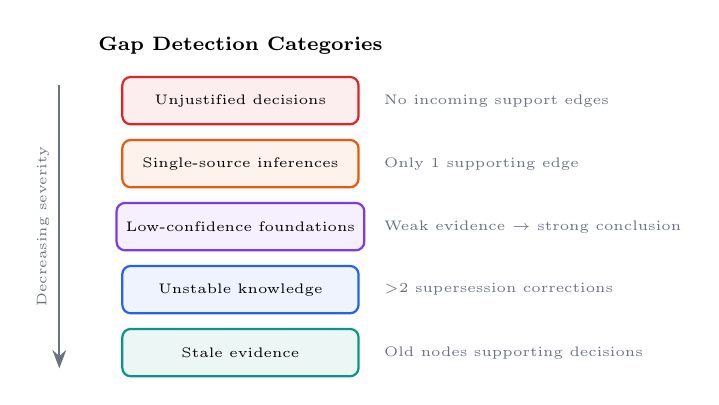
\begin{tikzpicture}[
  every node/.style={font=\tiny},
  gapbox/.style={rectangle, rounded corners=3pt, draw=#1, fill=#1!8, minimum width=3.0cm, minimum height=0.6cm, align=center, thick, font=\tiny},
]
\node[font=\scriptsize\bfseries] at (0, 0.5) {Gap Detection Categories};

\node[gapbox=amred] (g1) at (0, -0.2) {Unjustified decisions};
\node[font=\tiny, text=amgray, align=left, anchor=west] at (1.7, -0.2) {No incoming support edges};

\node[gapbox=amorange] (g2) at (0, -1.0) {Single-source inferences};
\node[font=\tiny, text=amgray, align=left, anchor=west] at (1.7, -1.0) {Only 1 supporting edge};

\node[gapbox=ampurple] (g3) at (0, -1.8) {Low-confidence foundations};
\node[font=\tiny, text=amgray, align=left, anchor=west] at (1.7, -1.8) {Weak evidence $\rightarrow$ strong conclusion};

\node[gapbox=amblue] (g4) at (0, -2.6) {Unstable knowledge};
\node[font=\tiny, text=amgray, align=left, anchor=west] at (1.7, -2.6) {$>$2 supersession corrections};

\node[gapbox=amteal] (g5) at (0, -3.4) {Stale evidence};
\node[font=\tiny, text=amgray, align=left, anchor=west] at (1.7, -3.4) {Old nodes supporting decisions};

% Severity arrow
\draw[amgray, thick, -{Stealth}] (-2.3, -0.0) -- (-2.3, -3.6) node[midway, left, font=\tiny, text=amgray, rotate=90, anchor=south] {Decreasing severity};

\end{tikzpicture}
\caption{Five categories of reasoning gaps detected by the gap detection query, ordered by default severity. Each gap type identifies a specific structural weakness in the agent's reasoning graph.}
\label{fig:gap_categories}
\end{figure}

% ----------------------------------------------------------------------------
\subsection{Cognitive Reasoning: Analogical Query}
\label{sec:analogy}

The analogical query finds past reasoning patterns structurally similar to a given target node's local subgraph. This implements a simplified form of structure-mapping~\cite{gentner1983structure} adapted for cognitive event graphs.

For each candidate node $c$, the algorithm computes:

\begin{equation}
\text{sim}(v, c) = 0.6 \cdot S_{\text{struct}}(v, c) + 0.4 \cdot S_{\text{content}}(v, c)
\label{eq:analogy}
\end{equation}

where $S_{\text{struct}}$ is based on the structural fingerprint---a vector of in-degree, out-degree, and edge-type distribution---and $S_{\text{content}}$ is cosine similarity between feature vectors (when available) or token overlap (as fallback).

The structural fingerprint for a node $v$ is:
\[
\mathbf{f}(v) = (\deg_{\text{in}}(v),\ \deg_{\text{out}}(v),\ h_1(v),\ h_2(v),\ \ldots,\ h_7(v))
\]
where $h_i(v)$ is the count of edges of type $i$ incident to $v$. Two fingerprints are compared by cosine similarity over these 9-dimensional vectors.

The query returns the top-$k$ analogous nodes (default $k = 5$), each annotated with the structural similarity score, content similarity score, and combined score. This enables an agent to ask: ``have I encountered a similar reasoning pattern before?'' and learn from past experience.


% ----------------------------------------------------------------------------
\subsection{Graph Maintenance: Consolidation}
\label{sec:consolidation}

The consolidation query performs four maintenance operations on the memory graph:

\begin{enumerate}[nosep, leftmargin=*]
  \item \textbf{Deduplication} --- Identifies node pairs with content similarity above a threshold (default: 0.9) based on token overlap. Duplicate pairs are reported with their similarity scores. In execute mode, the lower-confidence duplicate is linked to the higher-confidence one via a \textsc{Supersedes} edge.
  \item \textbf{Contradiction linking} --- Identifies fact nodes with contradictory content (detected by negation patterns and antonym heuristics) that lack \textsc{Contradicts} edges. In execute mode, missing contradiction edges are created.
  \item \textbf{Inference promotion} --- Identifies inference nodes with confidence above 0.9 that are supported by 3+ sources. These are candidates for promotion to fact status, reflecting the principle that well-supported inferences should be treated as established knowledge.
  \item \textbf{Orphan detection} --- Identifies nodes with no edges (neither incoming nor outgoing), which represent isolated knowledge fragments that may need integration or removal.
\end{enumerate}

A \emph{dry-run mode} reports what changes would be made without modifying the graph, enabling the agent (or user) to review proposed maintenance actions before committing them.

% ----------------------------------------------------------------------------
\subsection{Graph Maintenance: Drift Detection}
\label{sec:drift}

The drift detection query tracks how beliefs evolve over time by analyzing \textsc{Supersedes} chains and confidence trajectories.

For each topic cluster (identified by session or content similarity), the algorithm computes:

\begin{itemize}[nosep, leftmargin=*]
  \item \textbf{Stability score} --- The fraction of nodes in the cluster that have never been superseded. High stability indicates settled knowledge; low stability indicates an area of active revision.
  \item \textbf{Drift direction} --- Whether corrections trend toward higher or lower confidence, indicating whether the agent is becoming more or less certain about a topic.
  \item \textbf{Revision frequency} --- The rate of corrections per unit time, highlighting topics that are changing rapidly.
  \item \textbf{Trajectory} --- A chronological list of supersession events for each drifting belief, enabling the agent to see the full evolution of its understanding.
\end{itemize}

The output is a per-topic report ordered by instability, allowing the agent to focus attention on its least settled areas of knowledge.

% ----------------------------------------------------------------------------
\subsection{Summary of Algorithmic Complexity}

Table~\ref{tab:complexity} summarizes the algorithmic complexity and key data structures used by each new query type.

\begin{table}[t]
\caption{Algorithmic complexity and data structures for the nine new query types. $V$: nodes, $E$: edges, $q$: query terms, $P$: posting list size.}
\label{tab:complexity}
\centering
\scriptsize
\begin{tabular}{@{}lll@{}}
\toprule
\textbf{Query} & \textbf{Complexity} & \textbf{Key Structure} \\
\midrule
BM25 (fast) & $O(q \cdot |P|)$ & HashMap \\
BM25 (slow) & $O(V)$ & HashMap \\
Hybrid RRF & $O(V)$ & HashMap \\
PageRank & $O(k(V{+}E))$ & Vec \\
Degree centr. & $O(V{+}E)$ & HashMap \\
Betweenness & $O(V'E)$ & VecDeque \\
BFS shortest & $O(V{+}E)$ & VecDeque \\
Dijkstra & $O((V{+}E)\log V)$ & BinaryHeap \\
Belief revision & $O(V{+}E)$ & VecDeque \\
Gap detection & $O(V \cdot E)$ & HashMap \\
Analogical & $O(V^2)$ & Vec \\
Consolidation & $O(V^2)$ & HashMap \\
Drift detection & $O(V{+}E)$ & BTreeMap \\
\bottomrule
\end{tabular}
\end{table}


% ============================================================================
% 5. EVALUATION
% ============================================================================
\section{Evaluation}
\label{sec:evaluation}

We benchmark all nine new query types on synthetic graphs at 10K and 100K nodes using the Criterion statistical benchmarking framework (100 samples each) and single-run measurements for computationally intensive queries. The hardware, software, and dataset generation methodology match the v0.1 evaluation~\cite{owolabi2025agenticmemory}: Apple M4 Pro (ARM64), 64\,GB unified memory, Rust 1.90.0 with \texttt{--release} optimizations.

% ----------------------------------------------------------------------------
\subsection{Query Performance Overview}

Table~\ref{tab:allqueries} reports latency for all nine new query types on a 100{,}000-node graph (300K edges, 3 edges/node average). Queries span six orders of magnitude in latency, from 104\,$\mu$s (bidirectional BFS) to 297\,s (gap detection), reflecting fundamental differences in algorithmic complexity.

\begin{table}[t]
\caption{Query latency on 100K-node graph (Apple M4 Pro, release mode). Criterion benchmarks use 100 samples; single-run measurements marked with $\dagger$.}
\label{tab:allqueries}
\centering
\small
\begin{tabular}{@{}llr@{}}
\toprule
\textbf{Category} & \textbf{Query} & \textbf{Latency} \\
\midrule
\multirow{3}{*}{Retrieval} & BM25 (fast path) & 1.58\,ms \\
  & BM25 (slow path) & 122\,ms \\
  & Hybrid (BM25 + vector) & 10.83\,ms \\
\midrule
\multirow{5}{*}{Structure} & PageRank ($\alpha{=}0.85$) & 34.3\,ms \\
  & Degree centrality & 20.7\,ms \\
  & Betweenness centrality & 10.1\,s \\
  & Shortest path (BFS) & 104\,$\mu$s \\
  & Shortest path (Dijkstra) & 17.6\,ms \\
\midrule
\multirow{3}{*}{Cognitive} & Belief revision & 53.4\,ms \\
  & Gap detection$^\dagger$ & 297\,s \\
  & Analogical query$^\dagger$ & 229\,s \\
\midrule
\multirow{2}{*}{Maintenance} & Consolidation (dry)$^\dagger$ & 43.6\,s \\
  & Drift detection & 68.4\,ms \\
\bottomrule
\end{tabular}
\end{table}

The results divide cleanly into three tiers (Figure~\ref{fig:three_tiers}):

\textbf{Interactive queries ($<$100\,ms).} BM25, hybrid search, PageRank, degree centrality, BFS, Dijkstra, belief revision, and drift detection all complete within interactive latency bounds. These are suitable for per-query execution during agent conversations.

\textbf{Periodic queries (1--60\,s).} Betweenness centrality (10.1\,s) and consolidation (43.6\,s) are too slow for interactive use but practical for periodic batch execution---e.g., running once per session or on a schedule.

\textbf{Offline queries ($>$60\,s).} Gap detection (297\,s) and analogical reasoning (229\,s) at 100K nodes exhibit super-linear scaling due to their $O(V \cdot E)$ and $O(V^2)$ core loops, respectively. These are designed for offline analysis of large memory graphs, or for interactive use on smaller graphs (both complete in under 3\,s at 10K nodes, as shown in Table~\ref{tab:scaling}).

% ----------------------------------------------------------------------------
\subsection{Index Acceleration: Fast vs.\ Slow Path}

Table~\ref{tab:retrieval} isolates the impact of the TermIndex on BM25 performance.

\begin{table}[t]
\caption{BM25 text search: fast path (TermIndex) vs.\ slow path (full scan).}
\label{tab:retrieval}
\centering
\small
\begin{tabular}{@{}lrrr@{}}
\toprule
\textbf{Graph Size} & \textbf{Fast Path} & \textbf{Slow Path} & \textbf{Speedup} \\
\midrule
10K nodes & 186\,$\mu$s & 8.59\,ms & 46$\times$ \\
100K nodes & 1.58\,ms & 122\,ms & 77$\times$ \\
\bottomrule
\end{tabular}
\end{table}

The inverted index provides a 77$\times$ speedup at 100K nodes, with the advantage growing as graph size increases because the fast path cost depends on posting list size (sub-linear in $n$) while the slow path is always $O(n)$. This validates the TermIndex as a critical investment for backward-compatible acceleration.

% ----------------------------------------------------------------------------
\subsection{Scaling Analysis}

Table~\ref{tab:scaling} reports latency at 10K and 100K nodes for all queries, revealing scaling behavior.

\begin{table}[t]
\caption{Query latency scaling from 10K to 100K nodes.}
\label{tab:scaling}
\centering
\scriptsize
\begin{tabular}{@{}lrrr@{}}
\toprule
\textbf{Query} & \textbf{10K} & \textbf{100K} & \textbf{Ratio} \\
\midrule
BM25 (fast) & 186\,$\mu$s & 1.58\,ms & 8.5$\times$ \\
Hybrid & 1.00\,ms & 10.83\,ms & 10.8$\times$ \\
PageRank & 2.53\,ms & 34.3\,ms & 13.6$\times$ \\
Degree centr. & 1.73\,ms & 20.7\,ms & 12.0$\times$ \\
Betweenness & 6.43\,s & 10.1\,s & 1.6$\times$ \\
BFS & 7.9\,$\mu$s & 104\,$\mu$s & 13.2$\times$ \\
Dijkstra & 888\,$\mu$s & 17.6\,ms & 19.8$\times$ \\
Belief revision & 6.26\,ms & 53.4\,ms & 8.5$\times$ \\
Gap detection & 1.53\,s & 297\,s & 194$\times$ \\
Analogical & 2.40\,s & 229\,s & 95$\times$ \\
Consolidation & 352\,ms & 43.6\,s & 124$\times$ \\
Drift detect. & 5.84\,ms & 68.4\,ms & 11.7$\times$ \\
\bottomrule
\end{tabular}
\end{table}

Figure~\ref{fig:scaling_ratios} visualizes the scaling ratios for all queries. Queries fall into two scaling classes. \emph{Near-linear scalers} (ratio $\approx$10$\times$ for a 10$\times$ size increase): BM25, hybrid, PageRank, degree, BFS, Dijkstra, belief revision, and drift detection. These exhibit $O(n)$ or $O(n \log n)$ behavior and remain practical at scale. \emph{Super-linear scalers} (ratio $\gg$10$\times$): gap detection (194$\times$), consolidation (124$\times$), and analogical (95$\times$). These contain $O(n \cdot k)$ inner loops where $k$ grows with graph density, producing $O(n^2)$ or worse behavior on dense graphs. The betweenness centrality ratio (1.6$\times$) appears anomalous because Brandes' algorithm samples a fixed number of sources regardless of graph size; its absolute cost remains high (10.1\,s) due to the BFS cost per source on denser graphs.

% Figure: Three-tier classification
\begin{figure}[t]
\centering
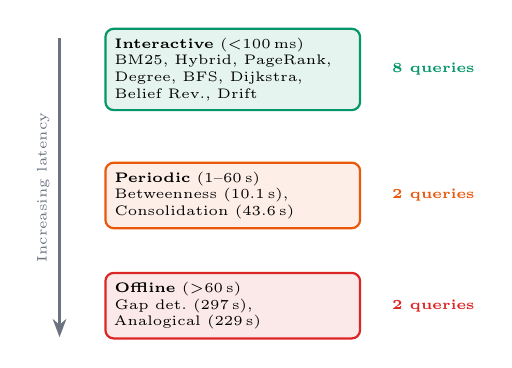
\begin{tikzpicture}[
  every node/.style={font=\tiny},
  tier/.style={rectangle, rounded corners=3pt, draw=#1, fill=#1!10, minimum width=3.2cm, minimum height=0.55cm, align=left, thick, font=\tiny, text width=3.0cm},
]

\node[tier=amgreen] (t1) at (0, 0) {\textbf{Interactive} ($<$100\,ms)\\BM25, Hybrid, PageRank,\\Degree, BFS, Dijkstra,\\Belief Rev., Drift};
\node[tier=amorange] (t2) at (0, -1.6) {\textbf{Periodic} (1--60\,s)\\Betweenness (10.1\,s),\\Consolidation (43.6\,s)};
\node[tier=amred] (t3) at (0, -3.0) {\textbf{Offline} ($>$60\,s)\\Gap det.\ (297\,s),\\Analogical (229\,s)};

% Count annotations
\node[font=\tiny\bfseries, text=amgreen, anchor=west] at (1.9, 0) {8 queries};
\node[font=\tiny\bfseries, text=amorange, anchor=west] at (1.9, -1.6) {2 queries};
\node[font=\tiny\bfseries, text=amred, anchor=west] at (1.9, -3.0) {2 queries};

% Arrow showing latency increase
\draw[amgray, thick, -{Stealth}] (-2.2, 0.4) -- (-2.2, -3.4) node[midway, left, font=\tiny, text=amgray, rotate=90, anchor=south] {Increasing latency};

\end{tikzpicture}
\caption{Three-tier query classification at 100K nodes. Eight of thirteen queries complete within interactive latency, making them suitable for per-query execution during agent conversations. Periodic and offline queries are designed for batch execution.}
\label{fig:three_tiers}
\end{figure}

% Figure: Scaling ratios bar chart
\begin{figure}[t]
\centering
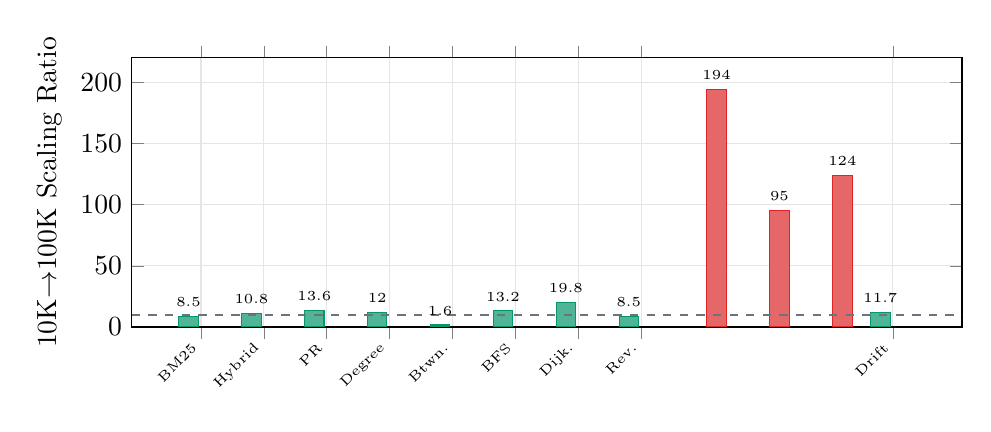
\begin{tikzpicture}
\begin{axis}[
  width=\columnwidth,
  height=5cm,
  ybar,
  bar width=7pt,
  xlabel={},
  ylabel={10K$\rightarrow$100K Scaling Ratio},
  symbolic x coords={BM25, Hybrid, PR, Degree, Btwn., BFS, Dijk., Rev., Gaps, Anal., Cons., Drift},
  xtick=data,
  xticklabel style={rotate=45, anchor=east, font=\tiny},
  ymin=0,
  ymax=220,
  grid=major,
  grid style={gray!20},
  nodes near coords,
  every node near coord/.append style={font=\tiny, anchor=south},
  point meta=explicit symbolic,
]
% Near-linear (green)
\addplot[fill=amgreen!70, draw=amgreen] coordinates {
  (BM25, 8.5) [8.5]
  (Hybrid, 10.8) [10.8]
  (PR, 13.6) [13.6]
  (Degree, 12.0) [12]
  (Btwn., 1.6) [1.6]
  (BFS, 13.2) [13.2]
  (Dijk., 19.8) [19.8]
  (Rev., 8.5) [8.5]
  (Drift, 11.7) [11.7]
};
% Super-linear (red)
\addplot[fill=amred!70, draw=amred] coordinates {
  (Gaps, 194) [194]
  (Anal., 95) [95]
  (Cons., 124) [124]
};
\draw[amgray, dashed, thick] ({rel axis cs:0,0}|-{axis cs:BM25,10}) -- ({rel axis cs:1,0}|-{axis cs:BM25,10}) node[right, font=\tiny, text=amgray] {Linear};
\end{axis}
\end{tikzpicture}
\caption{Scaling ratio (latency at 100K / latency at 10K) for each query. A ratio of 10 indicates linear scaling (dashed line). Queries below or near this line are practical at any graph size. Gap detection (194$\times$), consolidation (124$\times$), and analogical (95$\times$) exhibit super-linear scaling.}
\label{fig:scaling_ratios}
\end{figure}

% Figure: Performance comparison chart
\begin{figure}[t]
\centering
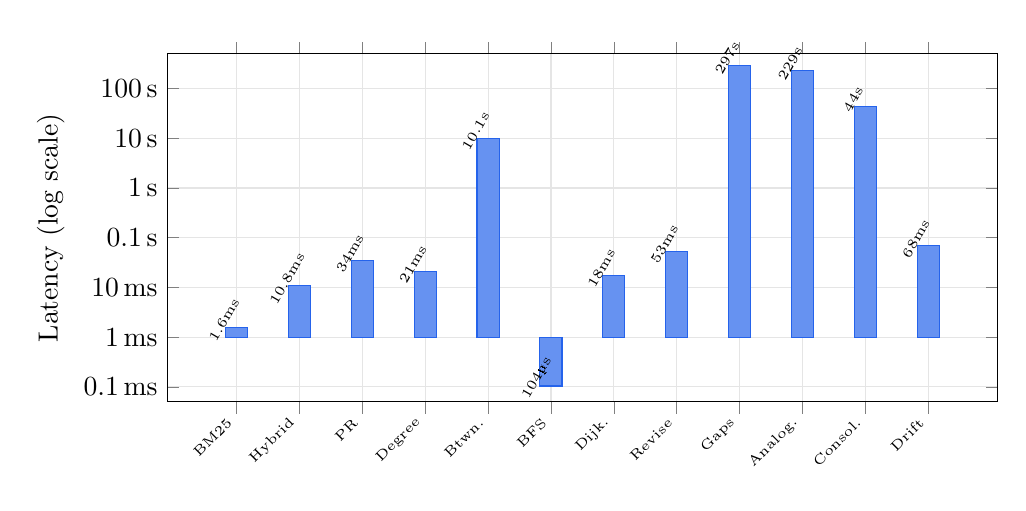
\begin{tikzpicture}
\begin{axis}[
  width=\columnwidth,
  height=6cm,
  ybar,
  bar width=8pt,
  xlabel={},
  ylabel={Latency (log scale)},
  ymode=log,
  log basis y=10,
  symbolic x coords={BM25, Hybrid, PR, Degree, Btwn., BFS, Dijk., Revise, Gaps, Analog., Consol., Drift},
  xtick=data,
  xticklabel style={rotate=45, anchor=east, font=\tiny},
  ytick={0.1, 1, 10, 100, 1000, 10000, 100000, 1000000},
  yticklabels={0.1\,ms, 1\,ms, 10\,ms, 0.1\,s, 1\,s, 10\,s, 100\,s, },
  ymin=0.05,
  ymax=500000,
  grid=major,
  grid style={gray!20},
  nodes near coords,
  every node near coord/.append style={font=\tiny, anchor=south, rotate=60},
  point meta=explicit symbolic,
]
\addplot[fill=amblue!70, draw=amblue] coordinates {
  (BM25, 1.58) [1.6ms]
  (Hybrid, 10.83) [10.8ms]
  (PR, 34.3) [34ms]
  (Degree, 20.7) [21ms]
  (Btwn., 10100) [10.1s]
  (BFS, 0.104) [{104\textmu s}]
  (Dijk., 17.6) [18ms]
  (Revise, 53.4) [53ms]
  (Gaps, 297000) [297s]
  (Analog., 229000) [229s]
  (Consol., 43600) [44s]
  (Drift, 68.4) [68ms]
};
\end{axis}
\end{tikzpicture}
\caption{Query latency across all nine new query types on a 100K-node graph (log scale). Six queries complete under 100\,ms (interactive). Gap detection, analogical reasoning, and consolidation require seconds to minutes, indicating they are suited for periodic or offline execution at this scale.}
\label{fig:all_query_latency}
\end{figure}

Figure~\ref{fig:scaling} plots latency at 10K and 100K for the interactive-tier queries on a log--log scale.

\begin{figure}[t]
\centering
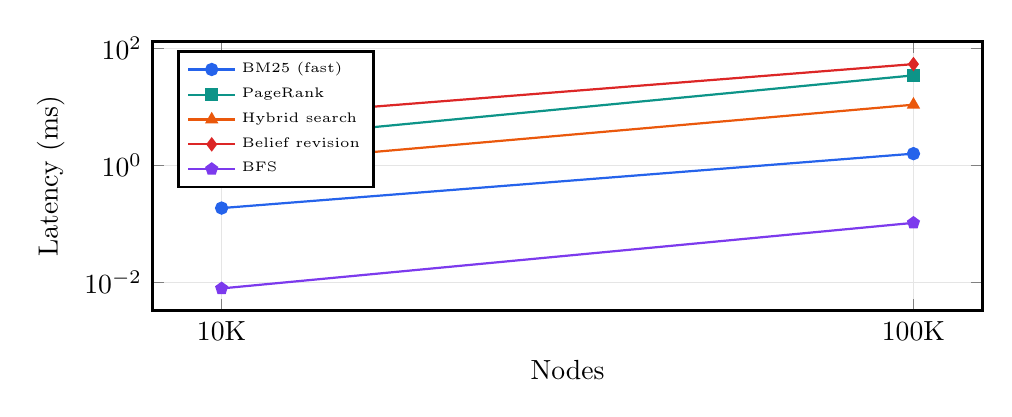
\begin{tikzpicture}
\begin{axis}[
  width=\columnwidth,
  height=5cm,
  xlabel={Nodes},
  ylabel={Latency (ms)},
  xmode=log,
  ymode=log,
  log basis x=10,
  log basis y=10,
  grid=major,
  grid style={gray!20},
  line width=1pt,
  mark size=2pt,
  xtick={10000, 100000},
  xticklabels={10K, 100K},
  legend pos=north west,
  legend style={font=\tiny, cells={anchor=west}},
]
\addplot[color=amblue, mark=*, thick] coordinates {
  (10000, 0.186) (100000, 1.58)
};
\addlegendentry{BM25 (fast)}

\addplot[color=amteal, mark=square*, thick] coordinates {
  (10000, 2.53) (100000, 34.3)
};
\addlegendentry{PageRank}

\addplot[color=amorange, mark=triangle*, thick] coordinates {
  (10000, 1.0) (100000, 10.83)
};
\addlegendentry{Hybrid search}

\addplot[color=amred, mark=diamond*, thick] coordinates {
  (10000, 6.26) (100000, 53.4)
};
\addlegendentry{Belief revision}

\addplot[color=ampurple, mark=pentagon*, thick] coordinates {
  (10000, 0.0079) (100000, 0.104)
};
\addlegendentry{BFS}

\end{axis}
\end{tikzpicture}
\caption{Scaling of interactive-tier queries from 10K to 100K nodes (log--log). All five queries exhibit near-linear scaling, remaining under 100\,ms at 100K nodes.}
\label{fig:scaling}
\end{figure}


% ============================================================================
% 6. PYTHON SDK
% ============================================================================
\section{Python SDK Extensions}
\label{sec:sdk}

The Python SDK (\texttt{pip install agentic-brain}) exposes all nine new queries through the \texttt{Brain} class, maintaining the zero-dependency design principle: the SDK communicates with the Rust engine via CLI subprocess calls and JSON serialization.

% ----------------------------------------------------------------------------
\subsection{New Brain Methods}

Nine new methods map directly to the query types:

\begin{lstlisting}[language=Python, caption={Python SDK methods for the nine new query types.}]
brain = Brain("agent.amem")

# Retrieval
results = brain.search_text("API rate limit")
results = brain.search("caching strategy",
                        top_k=10)

# Structural analysis
scores = brain.centrality(metric="pagerank")
path   = brain.shortest_path(src=42, dst=99)

# Cognitive reasoning
report = brain.revise(node_id=42)
gaps   = brain.gaps()
matches = brain.analogy(node_id=42, top_k=5)

# Maintenance
report = brain.consolidate(dry_run=True)
drift  = brain.drift()
\end{lstlisting}

Each method returns a typed dataclass from \texttt{agentic\_memory.results}: \texttt{TextMatch}, \texttt{HybridMatch}, \texttt{PathResult}, \texttt{RevisionReport}, \texttt{GapReport}, \texttt{Analogy}, \texttt{ConsolidationReport}, and \texttt{DriftReport}. These provide structured access to query outputs with named fields, type hints, and docstrings.

% ----------------------------------------------------------------------------
\subsection{Test Coverage}

The v0.2 Python SDK includes 104~tests across 8 test modules:

\begin{table}[t]
\caption{Python SDK test distribution across modules.}
\label{tab:python_tests}
\centering
\small
\begin{tabular}{@{}lr@{}}
\toprule
\textbf{Module} & \textbf{Tests} \\
\midrule
test\_brain.py & 30 \\
test\_query\_expansion.py & 20 \\
test\_models.py & 18 \\
test\_integrations.py & 12 \\
test\_agent.py & 8 \\
test\_cli\_bridge.py & 7 \\
test\_package.py & 7 \\
conftest.py (fixtures) & 2 \\
\midrule
\textbf{Total} & \textbf{104} \\
\bottomrule
\end{tabular}
\end{table}

The \texttt{test\_query\_expansion.py} module specifically validates all nine new methods with a \texttt{populated\_brain} fixture that creates a graph of 7~nodes across 3~sessions with typed edges. Tests cover: parameter validation, result type verification, empty-graph edge cases, event-type filtering, and metric selection.


% ============================================================================
% 7. IMPLEMENTATION
% ============================================================================
\section{Implementation Summary}
\label{sec:implementation}

Table~\ref{tab:implementation} summarizes the implementation effort for v0.2.

\begin{table}[t]
\caption{Implementation metrics for the v0.2 query expansion.}
\label{tab:implementation}
\centering
\small
\begin{tabular}{@{}lr@{}}
\toprule
\textbf{Metric} & \textbf{Value} \\
\midrule
New Rust code (query algorithms) & 3{,}586 lines \\
Total Rust code (engine) & 9{,}688 lines \\
Total Python SDK code & 2{,}298 lines \\
Rust tests (total) & 179 \\
Python tests (total) & 104 \\
New external dependencies & 0 \\
New CLI commands & 9 \\
New Python Brain methods & 9 \\
New result dataclasses & 8 \\
\bottomrule
\end{tabular}
\end{table}

\textbf{Zero new dependencies.} All graph algorithms---PageRank iteration, Brandes' betweenness centrality, bidirectional BFS, Dijkstra's algorithm, BM25 scoring, RRF fusion, structural fingerprinting, and cascade propagation---are implemented using only \texttt{std::collections} types (\texttt{HashMap}, \texttt{HashSet}, \texttt{BinaryHeap}, \texttt{VecDeque}, \texttt{BTreeMap}). This maintains the self-contained binary philosophy established in v0.1: the \texttt{amem} CLI has no runtime dependencies beyond the operating system.

\textbf{Nine new CLI commands.} Each query type is exposed as a CLI subcommand: \texttt{amem text-search}, \texttt{amem hybrid-search}, \texttt{amem centrality}, \texttt{amem path}, \texttt{amem revise}, \texttt{amem gaps}, \texttt{amem analogy}, \texttt{amem consolidate}, and \texttt{amem drift}. All commands support \texttt{--json} output for programmatic consumption by the Python SDK.

% ============================================================================
% 8. DISCUSSION
% ============================================================================
\section{Discussion}
\label{sec:discussion}

\textbf{From memory store to reasoning engine.} The v0.1 query model treated the memory graph as a navigable store: retrieve a node, follow its edges, find similar nodes. The v0.2 queries enable a qualitatively different mode of interaction: the agent can now analyze the \emph{structure} of its knowledge (centrality, shortest paths), audit the \emph{quality} of its reasoning (gap detection, belief revision), and \emph{maintain} its knowledge base autonomously (consolidation, drift detection). This transforms AgenticMemory from a persistence layer into a cognitive reasoning substrate.

\textbf{Cognitive gap detection as self-reflection.} The gap detection query is particularly novel in the context of agent memory. By identifying unjustified decisions, single-source inferences, and low-confidence foundations, it enables a form of epistemic self-reflection: the agent can assess the quality of its own reasoning without external supervision. This is related to metacognitive monitoring in cognitive science~\cite{flavell1979metacognition} and could support more calibrated decision-making in autonomous agents. The query is computationally expensive at 100K nodes (297\,s) due to its $O(V \cdot E)$ analysis of support chains, but completes in 1.5\,s at 10K nodes---fast enough for end-of-session execution. A natural optimization is incremental gap detection that only re-evaluates nodes modified since the last run.

\textbf{Analogical reasoning: offline at scale, interactive at moderate scale.} The analogical query enables a form of case-based reasoning~\cite{kolodner1992casebased} over the agent's entire history. By finding structurally similar past reasoning patterns, the agent can transfer lessons learned from previous situations to novel ones. The structural fingerprint approach captures meaningful structural similarity beyond surface-level text matching, but its $O(V^2)$ pairwise comparison loop makes it expensive at scale: 229\,s at 100K nodes (Table~\ref{tab:allqueries}). At 10K nodes---a practical size for single-agent memory accumulated over weeks of use---analogical search completes in 2.4\,s, making it viable as a periodic batch operation. Approximate nearest-neighbor indexes over structural fingerprints would reduce this to sub-second even at 100K nodes.

\textbf{Backward compatibility as a design principle.} The tag-length-value index block and feature-flags mechanism demonstrate that binary formats can evolve without breaking compatibility. This is particularly important for agent memory, where files may persist for months or years and be accessed by different versions of the software. The slow-path fallback ensures that new queries always work, albeit more slowly, on old files.

\textbf{Scalability tiers.} The benchmarks reveal a clear three-tier scalability picture. Eight of thirteen queries remain interactive ($<$100\,ms) at 100K nodes. Betweenness centrality (10.1\,s) and consolidation (43.6\,s) are periodic-tier operations. Gap detection (297\,s) and analogical reasoning (229\,s) are offline-tier at 100K nodes due to super-linear scaling (194$\times$ and 95$\times$ ratios for a 10$\times$ size increase, respectively). Practical agent memory graphs---typically 1K--20K nodes accumulated over weeks of interactions---fall comfortably within interactive range for all queries.

\textbf{Other limitations.} The BM25 tokenizer is a simple whitespace-and-punctuation splitter; a more sophisticated tokenizer (stemming, subword decomposition) would improve recall for morphological variants. Betweenness centrality with exact computation is $O(VE)$, which is impractical for graphs exceeding 100K nodes; our sampling approximation trades accuracy for speed. The consolidation deduplication uses token overlap rather than semantic similarity, which may miss paraphrases. The drift detection currently identifies instability but does not predict future drift trajectories.

\textbf{Future work.} Promising extensions include: (1)~approximate nearest-neighbor indexes for faster analogical search, (2)~incremental PageRank updates that avoid full recomputation when nodes are added, (3)~semantic deduplication using the existing feature vectors, (4)~temporal pattern mining to detect recurring reasoning cycles, and (5)~integration with LLM self-correction loops where gap detection triggers targeted knowledge acquisition.

% ============================================================================
% 9. CONCLUSION
% ============================================================================
\section{Conclusion}
\label{sec:conclusion}

We have presented AgenticMemory~v0.2.0, extending the binary graph memory format introduced in~\cite{owolabi2025agenticmemory} with nine new query types spanning retrieval, structural analysis, cognitive reasoning, and graph maintenance. The expansion is implemented in 3{,}586~lines of Rust with zero new dependencies, maintaining the self-contained design philosophy of the original system.

The new queries transform AgenticMemory from a navigable memory store into a cognitive reasoning engine. BM25 and hybrid search provide keyword-based retrieval complementing existing vector similarity. PageRank, betweenness centrality, and shortest-path algorithms reveal the topological structure of the agent's knowledge. Counterfactual belief revision, reasoning gap detection, and analogical pattern matching enable epistemic self-reflection. Consolidation and drift detection support autonomous knowledge maintenance.

Criterion benchmarks on 100{,}000-node graphs show that eight of thirteen queries complete within interactive latency ($<$100\,ms), with BM25 search at 1.58\,ms and bidirectional BFS at 104\,$\mu$s. Computationally intensive queries---gap detection (297\,s) and analogical reasoning (229\,s) at 100K nodes---are designed for periodic or offline execution and remain interactive at typical agent memory sizes ($<$20K nodes). Backward compatibility ensures that v0.1 files remain fully functional with v0.2 software via slow-path fallback (77$\times$ slower for BM25 without the TermIndex, but correct), and that v0.2 files degrade gracefully when read by v0.1 software via tag skipping and feature flags.

The complete system---9{,}688~lines of Rust, 2{,}298~lines of Python, 283~tests---demonstrates that sophisticated graph analytics can be embedded directly in an agent's memory layer without external services, databases, or cloud dependencies. Together with the foundation established in~\cite{owolabi2025agenticmemory}, AgenticMemory~v0.2.0 provides a complete cognitive memory substrate: persistent, portable, navigable, analytically rich, and entirely self-contained.


% ============================================================================
% REFERENCES
% ============================================================================
\bibliographystyle{plain}
\bibliography{references}

\end{document}
